\documentclass{article} 

\usepackage{fancyhdr}
\usepackage[english]{babel}

\usepackage{fullpage}
\usepackage[margin = .75 in]{geometry}
\usepackage[leqno]{amsmath}
\usepackage{amsmath}
\usepackage{amsfonts}
\usepackage{amssymb}
\usepackage{amsthm}
\usepackage{amssymb}
\usepackage[all]{xy}
\usepackage{graphicx}

\usepackage{graphicx,color,url,hyperref}
\usepackage{epsfig}
\fancyhf{}
\setlength{\parindent}{0pt}
\setlength{\parskip}{5pt plus 1pt}
\setlength{\headheight}{13.6pt}

\newcommand{\NN}{\mathbf N}
\newcommand{\RR}{\mathbf R}
\newcommand{\CC}{\mathbf C}
\newcommand{\ZZ}{\mathbf Z}
\newcommand{\ZZn}[1]{\ZZ/{#1}\ZZ}
\newcommand{\QQ}{\mathbf Q}
\newcommand{\nn}{\mathbb N}
\newcommand{\rr}{\mathbb R}
\newcommand{\cc}{\mathbb C}
\newcommand{\zz}{\mathbb Z}
\newcommand{\zzn}[1]{\zz/{#1}\zz}
\newcommand{\qq}{\mathbb Q}
\newcommand{\calM}{\mathcal M}
\newcommand{\latex}{\LaTeX}
\newcommand{\tex}{\TeX}
\newcommand{\dd}{{\rm d}}
\newcommand{\sm}{\setminus} 

\title{Homework 3}
\author{Sunny Lee}
\date{March 30, 2021}

\pagestyle{fancy}
\fancyhf{}
\rhead{March 30, 2021}
\lhead{Sunny Lee}
\chead{Homework 3}
\rfoot{Page \thepage}

\begin{document}

\begin{enumerate}
    \item Let $\{a_n\}$ be a sequence of real numbers such that $|a_n| \leq 2$ and 
    $|a_{n+2} - a_{n+1}| \leq \frac{1}{8}|a_{n+1}^2 - a_n^2| \forall n\geq 1$. Then, 
    $\frac{1}{8}|a_{n+1}^2 - a_n^2| = \frac{1}{8}|(a_{n+1} - a_n)(a_{n+1} + a_n)|
    \leq \frac{1}{8^2}|a_n^2 - a_{n-1}^2||a_{n+1} + a_n| \leq \cdots \leq 
    \frac{1}{8^{n-2}}|a_2^2 - a_1^2||a_{n+1}+a_n|\cdots |a_3 + a_2|$. 
    Since $|a_n|\leq 2$, $\frac{1}{8^{n-2}}|a_2^2 - a_1^2||a_{n+1}+a_n|\cdots |a_3 + a_2|
    \leq \frac{1}{8^{n-2}}|a_2^2 - a_1^2||2+2|\cdots |2 + 2| = 
    \frac{1}{8^{n-2}}|a_2^2 - a_1^2|4^{n-2} = \frac{1}{2^{n-2}}|a_2^2 - a_1^2|$. Since 
    $\frac{1}{2^{n-2}}\rightarrow 0$ as $n\rightarrow \infty$, $\{a_n\}$ is Cauchy. Thus
    $\{a_n\}$ converges.

    \item For all $x, y \in \rr$, $|cos(x) - cos(y)| = 2|sin(\frac{x+y}{2})
    sin(\frac{x-y}{2})| \leq 2|sin(\frac{x-y}{2})| < 2|\frac{x-y}{2}| = |x-y|$. Thus, 
    if we let $\delta = \epsilon$, $|f(x) - f(y)| < \epsilon$ if $|x-y| < \delta$. Thus, 
    $f(x) = cos(x)$ is uniformly continuous on all of $\rr$. 

    \item Let $f(x) = cos(x)$ where $x\in \rr$. Then, $f'(x) = -sin(x)$ Since $sin(x)$
    is bounded by $[-1, 1]$, the derivative is bounded below by $-1$ and above by $1$. 
    Thus, $|f'| \leq 1$. Since $f$ is a function with a bounded derivative, $cos(x)$
    is continuous on all of $\rr$. 

    \item Since we are no longer in the interval $[-\pi, \pi]$, we must take back 
    into consideration $L$, our period. We also now have a disctoninuous piecewise 
    function and so when we are integrating, we must split our integral into two 
    parts. Taking this into account, we can write a script in Matlab to get our first
    four fourier series terms: \\
    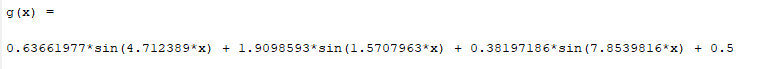
\includegraphics[scale = .9]{6.png}\\
    Plotting these four terms: \\
    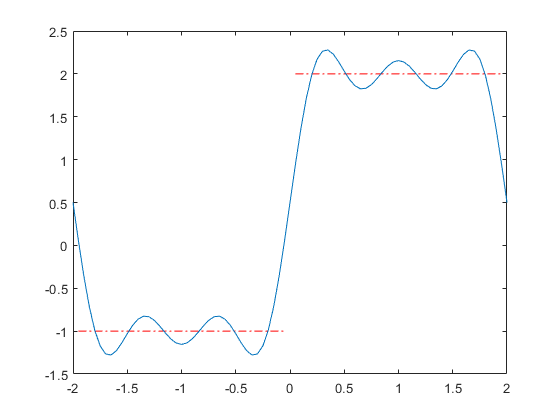
\includegraphics[scale = .7]{6plot.png}
\end{enumerate}

\end{document}